

\section{Evaluations} \label{Evaluation}

\begin{figure}
	\centering
	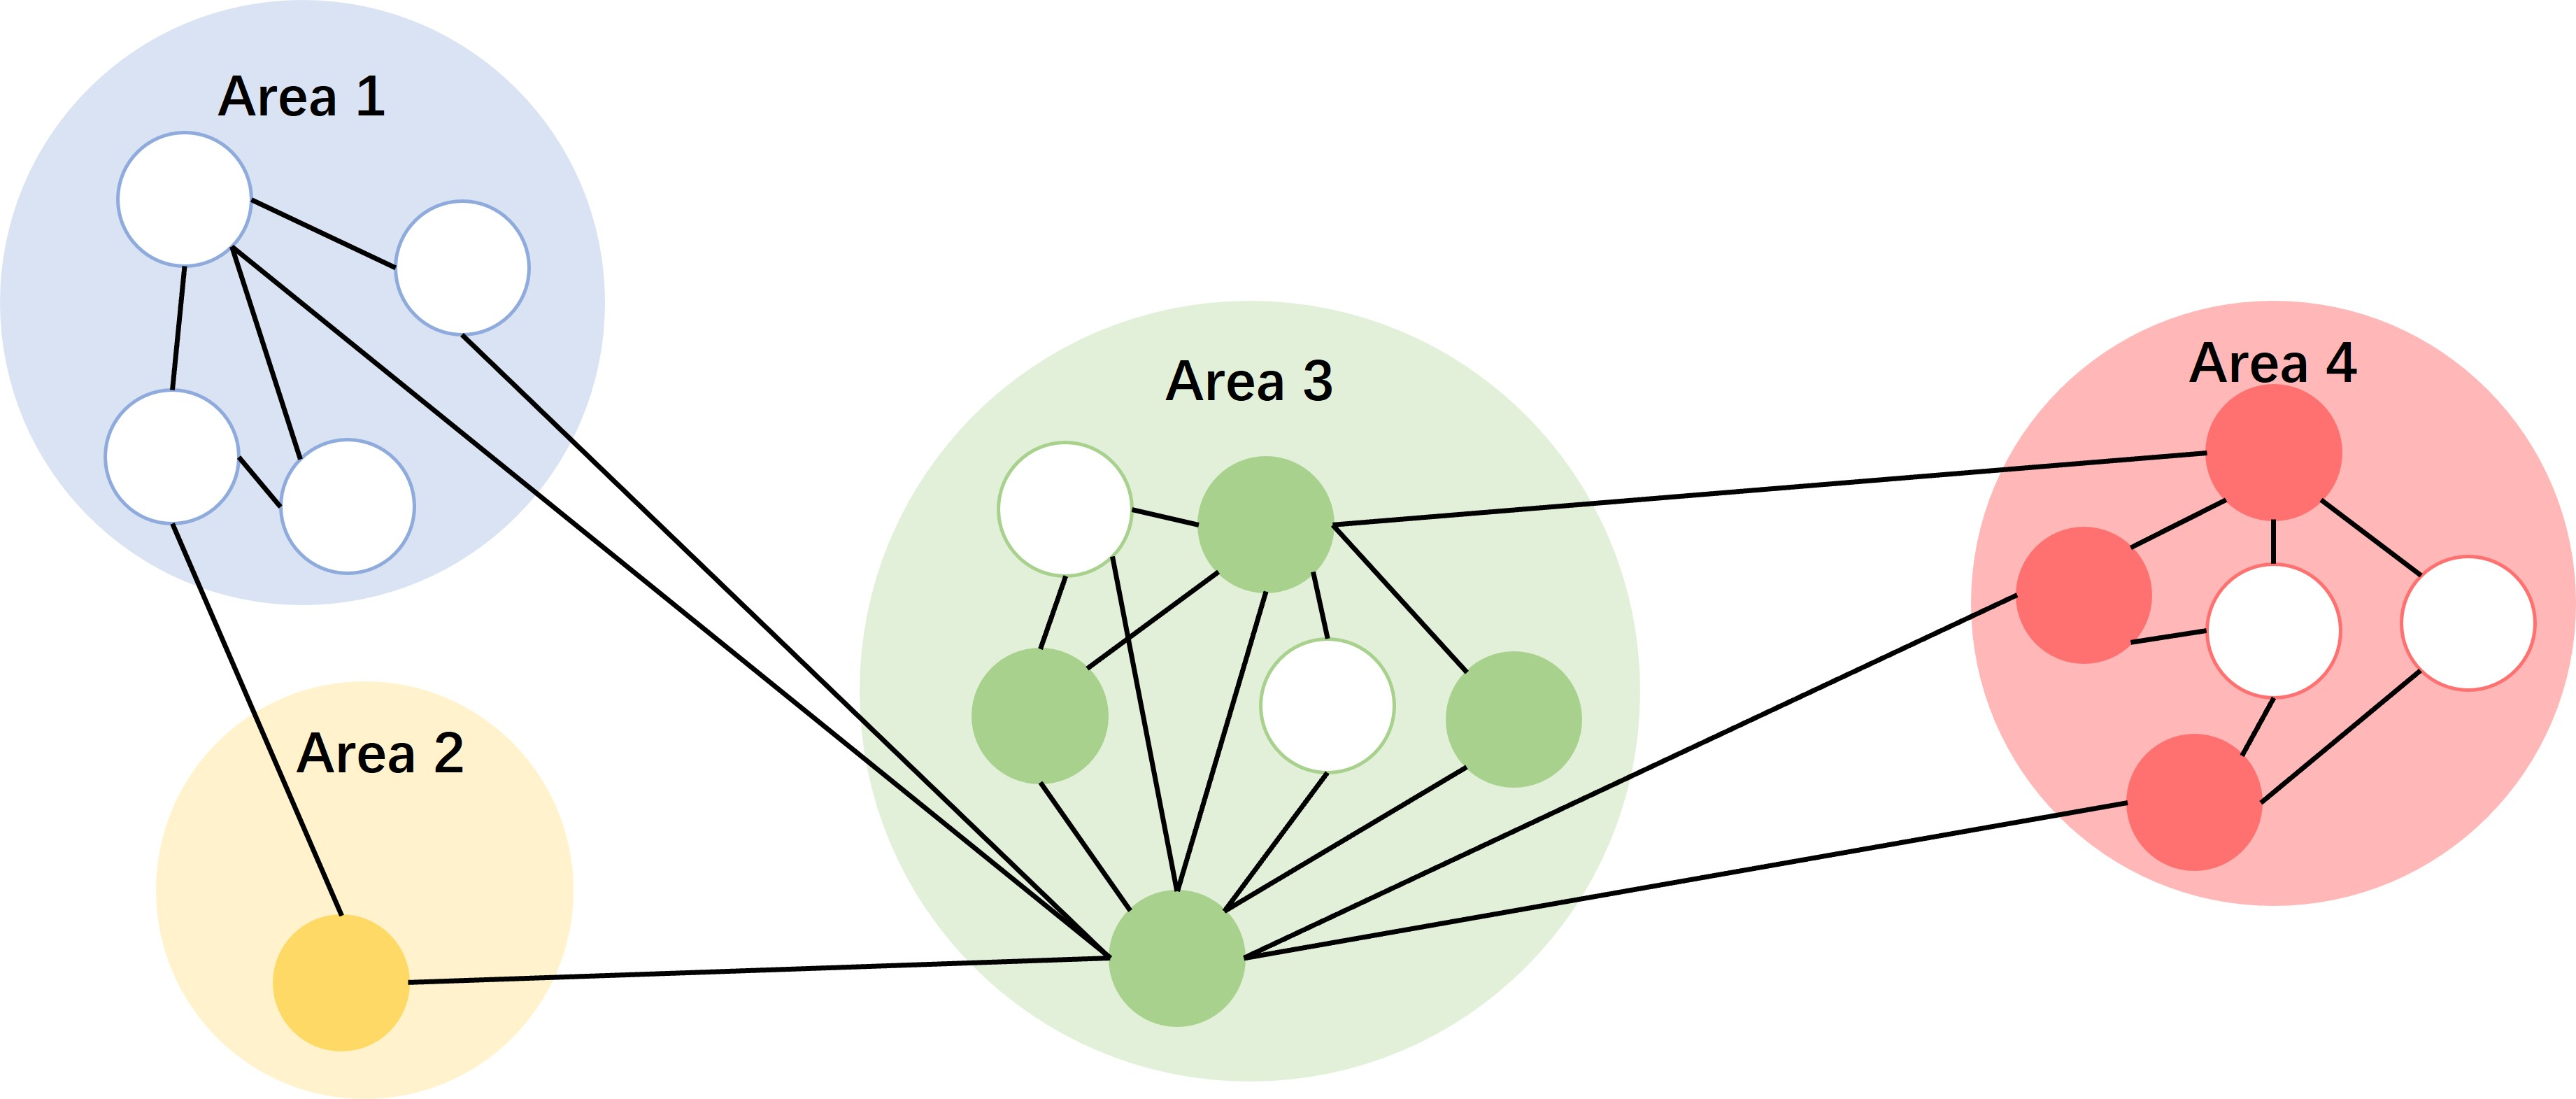
\includegraphics[width = 8cm]{figs/architecture/Topology.jpg}
	\caption{\small Shows the test topology consisting of 8 PoPs with programmable switches highlighted in color, and 8 PoPs without programmable switches marked in white}
	\label{fig:topo}
\end{figure}

As shown in Figure \ref{fig:topo}, the test input network topology includes 860 {\egresses}, among which there are 32 Transit {\egresses}, comprising 16 PoPs in total. 8 of these PoPs have programmable devices capable of detecting flows, while the other 8 PoPs act solely as transit PoPs, utilizing their backbone network links. The total number of backbone network links is 40. The amount of flows in the test input is approximately 2 million per time slot and the flows are all from real business traffic of 1 week (from May 22, 2023 to May 28, 2023). Performance-aware flows are marked according to the application service class, with the number being roughly 4\% of the total number of flows. The algorithm runs on a single server with 64GB of memory and 32 CPU cores.


% performance-aware flow identification and characteristics. 

There are two parameters to be determined. We filter non-performance-aware small flows based on a flow filter threshold $FT$. 
Considering the risk in practical deployments, we set the maximum percentage of {\egress} burst capacity as a hyperparameter burst threshold, denoted as $BT$, to prevent congestion at the {\egresses}.

% 其他论文的用词
% 冲顶 != burst
We compare the difference in scheduling results between {\sys} and existing network scheduling algorithm in terms of cost optimization and performace optimization. Existing approaches cannot be applied in our scenarios because none of the current algorithms that focus on cost and performance optimization scheduling take the capacity constraints of the backbone network as a limitation. We select the existing network controller’s traffic scheduling algorithm as the baseline algorithm. The baseline approach categorizes flows directed towards specific predetermined ASes as performance-aware flows. This baseline method switch reroutes the entire traffic trunks associated with the specified ASes from one {\egress} to another. However, this routing granularity is relatively coarse and this method does not optimize the final cost. We will show that {\sys} employs application service classes and destination ISP prefixes to identify flows, thereby optimizing final cost and performance-aware routing to better align with the specific performance requirements of clients.

To verify the effectiveness of the proposed algorithms. We first conduct tests on our algorithm's performance in cost optimization and performance optimization under various hyperparameters. Then we evaluate the algorithm's runtime under different number of threads in large-scale tests to show that it has good scalability. Finally, we discuss problems that may be encountered in the application of the algorithm.

% Nowadays, cloud providers consistently implement performance-aware routing at cloud's edge. The baseline approach categorizes flows directed towards specific predetermined ASes as performance-sensitive flows. This baseline method switch reroutes the entire traffic trunks associated with the specified ASes from one {\egress} to another. However, this routing granularity is relatively coarse.  Conversely, our proposed approach employs source application types and destination prefixes to identify flows, thereby optimizing performance-aware routing to better align with the specific performance requirements of clients.


% We select the baseline algorithm ... briefly explains the algorithm and reference \cite{iwqos, infocom}. % 给几个NSDI,SIGCOMM iwqos 
% We compare the scheduling results of {\sys} with the existing network controller’s traffic scheduling algorithm. 


\subsection{Cost Optimization} \label{Cost Optimization}

We first conducted offline tests for 1 to 7 days with hyperparameters such as a burst threshold of 90\% and a flow filter threshold of 0.1Mb. The test results are shown in Table \ref{tab:7days}, indicating that {\sys} exhibits relatively stable cost optimization compared to the existing network controller's traffic scheduling scheme, with an optimization ratio of approximately 36\%. Furthermore, as the number of time slots increases, {\sys} achieves greater cost optimization, suggesting that our algorithm possesses a certain level of stability. Given that the effect of cost optimisation is almost independent of the number of test slots, the number of test slots is set to the number of slots for 1 day, i.e. 288 slots, for all subsequent experimental tests.

\begin{table}[tbp]
%	\footnotesize
	\centering
  \resizebox{0.48\textwidth}{7mm}{
	\begin{tabular}{c|c|c|c|c|c|c|c}
		\hline
 Days & 1 & 2 & 3 & 4 & 5 & 6 & 7  \\ 
 \hline
 Baseline & 1080.09 &	1106.51 & 1137.02 & 1162.89 & 1173.52 & 1181.04 & 1187.20\\ 
 \hline
 {\sys}& 712.47 & 719.21 & 730.95 & 737.69 & 744.79 & 750.27 & 754.18  \\ 
 \hline
 Optimization & 34.04\% & 35.00\% & 35.71\% & 36.56\% &36.53\% & 36.47\% & 36.47\% \\ 
 \hline
	\end{tabular}
 }
        \vspace{-0.1in}
	\caption{\small Cost optimization for 1 to 7 days of offline testing under a 90\% burst threshold and a 0.1Mb flow filter threshold}
	\label{tab:7days}
\end{table}

We compared the cost optimization effects of {\sys} under different hyperparameters settings to the existing network scheduling algorithm, while keeping other experimental settings constant. Figure \ref{fig:costTestpara1} illustrates the relationship between the flow filter threshold and the percentage of cost savings under the same burst threshold. It shows that with a fixed burst threshold, the percentage of cost savings increases as the flow filter threshold decreases. However, when the flow filter threshold becomes sufficiently small (e.g., 0.1Mb), further decreasing the flow filter threshold does not significantly increase the final cost. It indicates that higher burst thresholds often result in a lower final cost. This is because the total bandwidth of the remaining flows does not decrease significantly as FT continues to decrease, thereby not yielding a substantial enhancement in cost optimization.

\begin{figure}
	\centering
	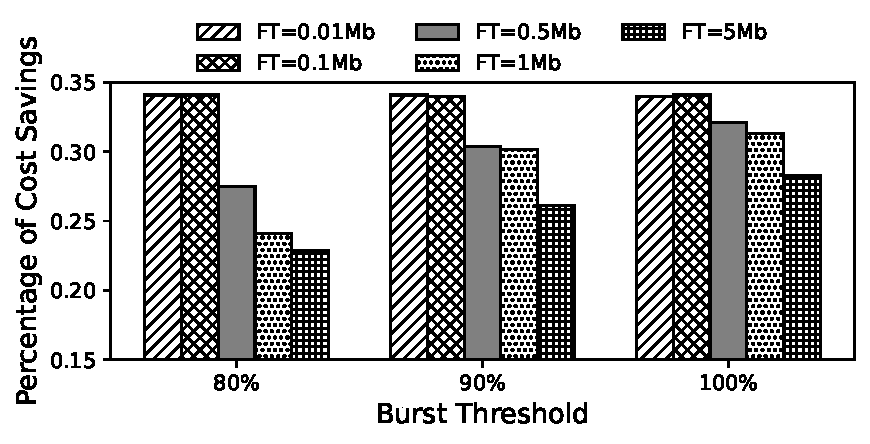
\includegraphics[width = 7cm]{figs/evaluation/costTestpara1.pdf}
	\caption{\small Impact of flow filter threshold on cost optimization when choosing different burst thresholds}
	\label{fig:costTestpara1}
\end{figure}


% \begin{figure}
% 	\centering
% 	\includegraphics[width=8cm]{figs/evaluation/plot2.pdf}
% 	\caption{\small test SVG figure}
% 	\label{fig:test}
% \end{figure}


\subsection{Performance Optimization}
Then, we test the performance optimization effect of {\sys} on performance-aware flows. We choose the delay of the flow to the {\egress} as the performance metric, which contains the {\egress} delay, and the backbone link delay. We compare the differences in latency performance optimization between the {\sys} scheduling algorithm and the existing network controller's scheduling algorithm for performance-aware flows. Our testbed settings are the same as mentioned earlier. We test for 288 time slots, with a burst threshold of 90\% and a flow filter threshold of 0.1Mb. Figure \ref{fig:performanceTestAbs} illustrates the variation of average latency for performance-aware flows over time slots under the two traffic scheduling schemes. {\sys}, compared to the existing network's traffic scheduling algorithm, reduces the average latency for performance-aware flows from 44.2ms to 41.7ms, achieving an absolute average decrease of about 2.5ms. We test the percentage of performance-aware flows optimized by {\sys} to the total performance-aware flows under each time slot. As shown in Figure \ref{fig:performanceTestPrecent}, in comparison to the existing network controller's scheduling algorithm, {\sys} can reduce the latency of approximately 67\% performance-aware flows.

\begin{figure}
	\centering
	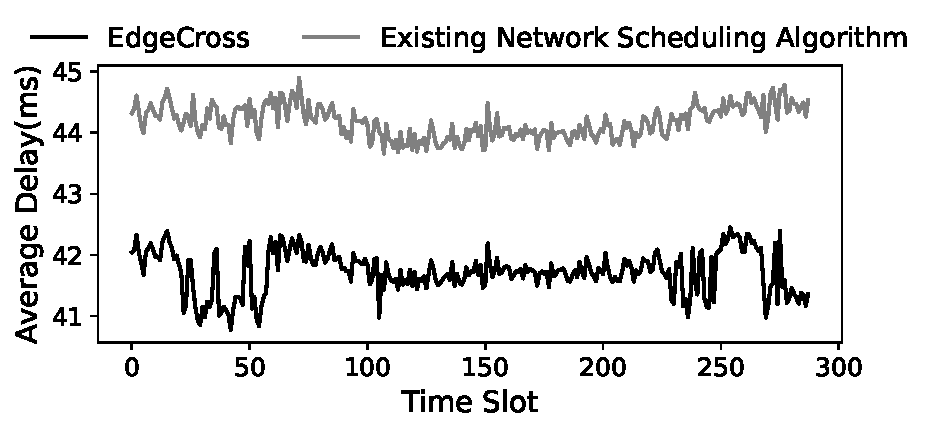
\includegraphics[width = 8cm]{figs/evaluation/performanceTestAbs.pdf}
	\caption{\small Comparison of average delay of performance-aware flows at each time slot under {\sys} and existing network scheduling algorithm}
	\label{fig:performanceTestAbs}
\end{figure}

\begin{figure}
	\centering
	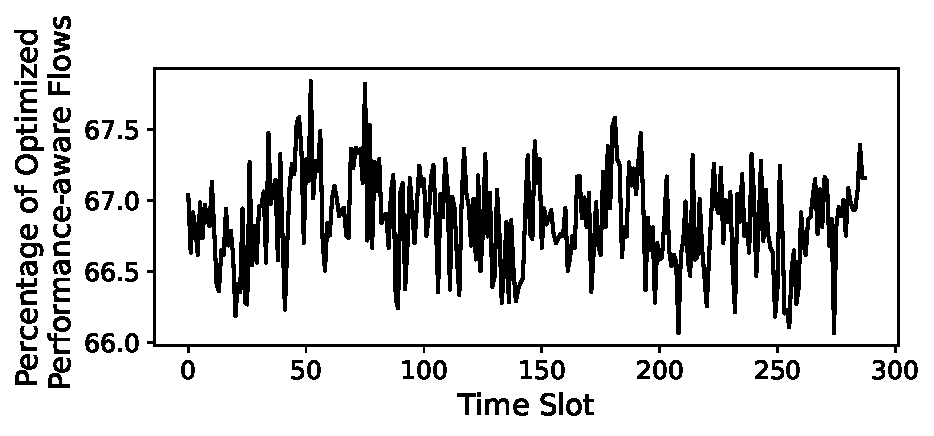
\includegraphics[width = 8cm]{figs/evaluation/performanceTestPrecent.pdf}
	\caption{\small Percentage of optimized performance-aware flows to total performance-aware flows at each time slot with {\sys} compare to existing network scheduling algorithm}
	\label{fig:performanceTestPrecent}
\end{figure}


The results are shown in Table \ref{fig:performanceTestHyperparameters}. It shows that different hyperparameters doesn't significantly affect the performance optimization for performance-aware flows. This is due to three main reasons: Firstly, {\sys} does not filter the perfromance-aware flows, which means flow filter threshold is unaffected to the performance. Secondly, our algorithm prioritizes optimizing the performance for performance-aware flows by a heuristic strategy; Thirdly, the number of performance-aware flows is relatively small and constitutes a small portion of the total flow size. So almost every performance-aware flow can be placed to the optimal {\egress}.


\iffalse
\begin{figure}
	\centering
	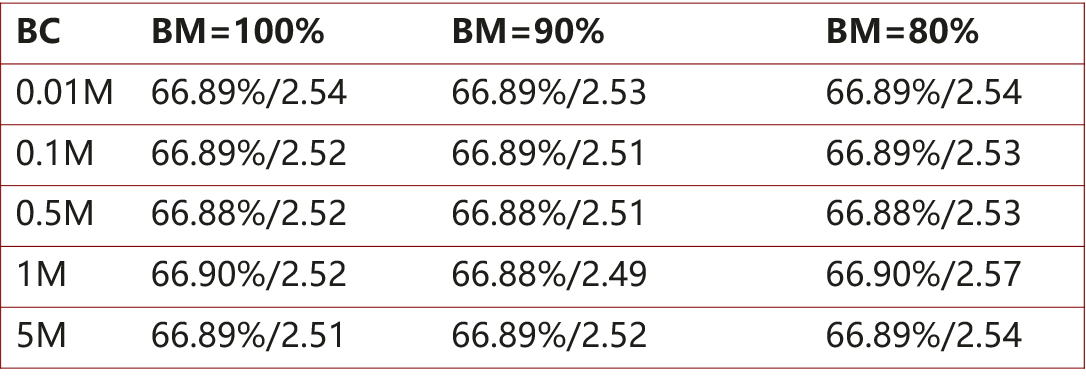
\includegraphics[width = 8cm]{figs/evaluation/performanceTestHyperparameters.png}
	\caption{\small Impact of choosing different hyperparameters on performance optimization}
	\label{fig:performanceTestHyperparameters}
\end{figure}
\fi

\begin{table}[tbp]
	\footnotesize
	\centering
{
	\begin{tabular}{c|c|c|c}
		\hline
 \diagbox{FT}{BT} & 100\% & 90\% & 80\%  \\ 
 \hline \hline 
 0.01 Mb & 66.89\% & 66.89\% & 66.89\%  \\ 
 \hline
 0.1 Mb  & 66.89\% & 66.89\% & 66.89\%  \\ 
 \hline
  0.5 Mb & 66.88\% & 66.88\% & 66.88\%  \\ 
   \hline
  1 Mb   & 66.90\% & 66.88\% & 66.90\%  \\ 
   \hline
  5 Mb   & 66.89\% & 66.89\% & 66.89\%  \\ 
 \hline
 \end{tabular}
 }
     \vspace{-0.1in}
	\caption{\small The ratio of performance-aware flows optimized for different hyperparameter combinations to the total number of performance-aware flows}
	\label{fig:performanceTestHyperparameters}
\end{table}

% 我们的算法在更大规模下是不是还适用
\subsection{Scalability}
Since {\sys}'s objective is to perform large-scale traffic scheduling, computational efficiency during online scheduling is of paramount importance. Following the same testbed setup as described earlier, we test the average runtime of the algorithm per time slot under different hyperparameters for the serial version. Table \ref{fig:runtimeHyper} shows that the burst threshold has almost no impact on the average runtime, as the average runtime is primarily determined by the large number of flows awaiting scheduling, and changing the burst threshold doesn't affect the number of flows. On the other hand, changes in the flow filter threshold significantly impact the average runtime of the algorithm. As the flow selection filter increases, fewer flows participate in the optimization scheduling, resulting in shorter algorithm runtime.

\begin{table}[tbp]
%	\footnotesize
	\centering
  \resizebox{0.48\textwidth}{13mm}{
	\begin{tabular}{c|c|c|c|c|c}
		\hline
 FT & BW PCT. & Number PCT. & BT=100\% & BT=90\% & BT=80\% \\ 
 \hline \hline 
 0 Mb & 100\% & 100\% & 30073.82 & 31720.58 & 29794.35 \\ 
 \hline
 0.01 Mb & 99.63\% & 13.33\% & 4734.45 & 4426.03 & 4479.67 \\ 
 \hline
 0.1 Mb & 99.22\% & 3.67\% & 1910.24 & 2074.08 & 1927.25 \\ 
 \hline
  0.5 Mb & 96.44\% & 1.42\% & 1794.02 & 1889.40 & 1764.48 \\ 
   \hline
  1 Mb & 89.10\% & 0.92\% & 1775.68 & 1767.36 & 1684.17 \\ 
   \hline
  5 Mb & 86.49\% & 0.35\% & 1652.33 & 1548.39 & 1586.25 \\ 
 \hline
 \end{tabular}
 }    
    \vspace{-0.1in}
	\caption{\small Impact of different hyperparameters on algorithm runtime under single threading(ms)}
	\label{fig:runtimeHyper}
\end{table}

Next, we scale up the number of flows by triplicating the Transit flows, bringing the flow number to around 5 million, and reduce the bandwidth of these flows to one-third of the original to keep the total bandwidth same. Besides, no flows are filtered, maintaining a flow count of around 5 million for scheduling, while other experimental settings remains consistent. We compare the average runtime of the algorithm per time slot under different number of threads. As shown in Figure \ref{fig:runtimeComp}, under the parallel 32-threaded mode, the algorithm's average runtime is approximately 80\% shorter than the serial mode. This indicates that if filtering is applied to flows with a flow filter threshold of 0.1Mb, our algorithm can support the scheduling of around 500 million flows within approximately 10 seconds with 32 threads.

% \begin{table}[tbp]
% %	\footnotesize
% 	\centering
%   \resizebox{0.48\textwidth}{7mm}{
% 	\begin{tabular}{c|c|c|c|c|c|c}
% 		\hline
%  Mode & Burst & Delay-Sensetive Flow & Inter-PoP & Intra-PoP & Remain Flows & Total \\ 
%  \hline \hline 
%  32 Parallel threads & 90.40 & 57.62 & 528.42 & 3356.14 & 6004.58 & 10037.16 \\ 
%  \hline
%  2 Parallel threads  & 90.28 & 56.55 & 1353.64 & 46104.40 & 15756.87 & 63361.74 \\ 
%  \hline
%  Serial & 96.82 & 41.88 & 44011.70 & 44011.70 & 11618.94 & 55769.34 \\ 
%  \hline
%  \end{tabular}
%  }
%         \vspace{-0.1in}
% 	\caption{\small Running time of individual components in different run modes(ms)}
% 	\label{fig:runtimeComp}
% \end{table}
\begin{figure}
	\centering
	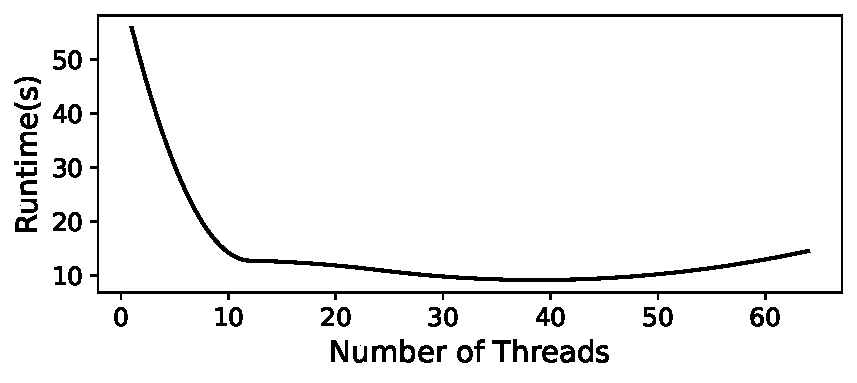
\includegraphics[width = 8cm]{figs/evaluation/runtimeComp.pdf}
	\caption{\small Running time per time slot of different number of threads under about 5 million flows(s)}
	\label{fig:runtimeComp}
\end{figure}



% \subsection{Hyperparameter Selection}






\subsection{Discussion}
\para{How to set the hyperparameters?} Based on the results of the tests mentioned above, we analyzed the impact of the two hyperparameters, the burst threshold $BT$ and the flow filter threshold $FT$, on the final optimization results. Cost optimization is influenced by both hyperparameters, while performance optimization is unaffected by them, and the algorithm's average runtime is influenced solely by the flow filter threshold. In order to maintain favorable cost optimization results and mitigate the risks associated with the upper bound of {\egress} capacity, we ultimately chose to set the burst threshold at 90\%. The choice of the flow filter threshold affects both optimizations simultaneously. Figure \ref{fig:hyperChoose} shows the percentage of cost savings and algorithm's average runtime under different flow filter thresholds. It can be told that as the flow filter threshold decreases from 5Mb to 0.1Mb, the final cost significantly reduces, while the algorithm's average runtime remains relatively stable. However, when the flow filter threshold is further reduced to 0.01Mb, the percentage of cost savings doesn't exhibit significant growth, while the algorithm's average runtime increases notably. Consequently, we settled on a flow filter threshold of 0.1Mb.

\begin{figure}
	\centering
	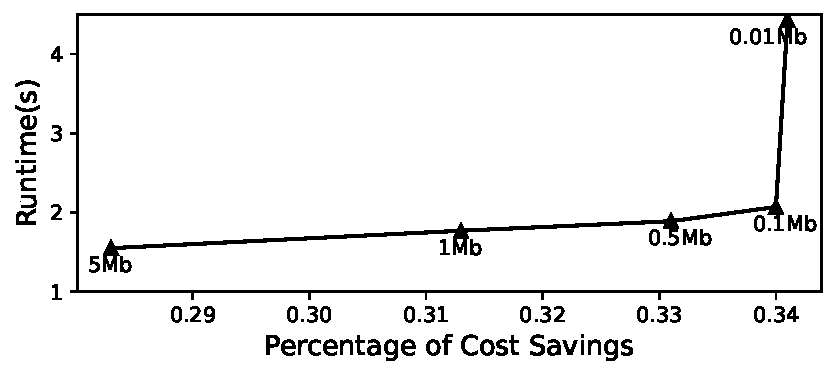
\includegraphics[width = 8cm]{figs/evaluation/hyperChoose.pdf}
	\caption{\small Percentage of cost savings and average running time of a single time slot under a single thread for different flow filter thresholds at 90\% of the burst threshold}
	\label{fig:hyperChoose}
\end{figure}

\para{What if the number of performance-aware flows is large?} When performance-aware flows dominate the bandwidth of the majority of flows in the network, {\sys} can still integrate cost and performance objectives for traffic scheduling. The reason is that performance-sensitive flows often tend to be scheduled within this PoP for better performance. Scheduling across PoPs offen impairs performance metrics such as delay and packet loss. However, the core of cost optimization lies in making full use of the suggested bandwidth of the backbone given by the solver, i.e. the virtual link capacity between PoPs. Therefore, if non-performance-aware flows are able to fully utilize the capacity of these virtual links, {\sys} can still well optimize the final cost. If the total available capacity of each intra-PoP {\egress} is greater than the total bandwidth of the performance-aware flows within the PoP, the perfomance of flows can still be optimized.

\para{What if the virtual link capacity is not utilized during heuristic scheduling?} We designed another simple heuristic scheduling algorithm to demonstrate the necessity of utilizing virtual link capacity. This algorithm schedules flows directly to a feasible {\egress} after arranging them in descending order of bandwidth. We evaluate the performance of this simple algorithm and {\sys} in terms of cost optimization. As shown in Figure \ref{fig:backboneEffect}, this heuristic algorithm can only optimize approximately 6\% of the cost, which is significantly lower than the optimization achieved by {\sys}. As analyzed in Section \ref{Solving Optimization Quickly}, the insufficient capacity of the backbone network results in the inability to route flows out of certain PoPs, causing a rapid growth in the {\egress} $p_i$ of these PoPs.

\begin{figure}
	\centering
	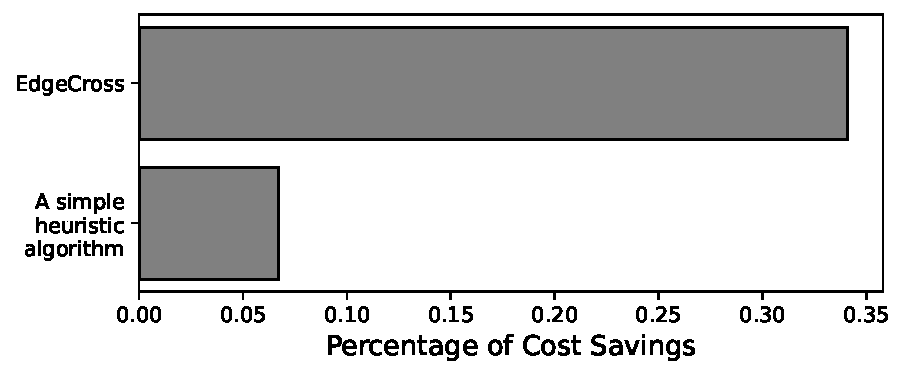
\includegraphics[width = 8cm]{figs/evaluation/backboneEffect.pdf}
	\caption{\small Comparing cost optimization between {\sys} and the simple heuristic algorithms using the hyperparameter settings $FT=0.1Mb$ and $BT=90\%$.}
	\label{fig:backboneEffect}
\end{figure}

% \para{What if the predicted charged bandwidth per {\egress} given by the overall level optimization is not accurate?} Since the {\egress} charge bandwidth prediction $p_i$ given by the overrall level optimization will act as a constraint when scheduling online, if the sum of the $p_i$ of all {\egresses} within a PoP is too low, 5\% of the burst time slots will be quickly exhausted. In this case, the actual final cost may be much higher than the overrall level prediction.


% \subsection{Robustness Analyze}
% \subsection{Tolerance}  Error Resilience Analysis 或者 Error Tolerance Analysis  叫作误差容忍性分析
% 分析对于预测的敏感程度 和 预测偏差的容忍度
% 1. 如果总体层面不那么准
% 2. 如果预测的总带宽和PoP的带宽趋势不那么准(每个月的带宽增加是在这里,但如果预测的和这个月的带宽增加不一样的,那就要查看这个)
% 3. 如果时隙层面的流不那么准
% 4. 如果时隙层面的PoP带宽直接用上一个时隙的

% 如果有突发的大流,如何处理不会使得成本 prohibitively raise
% \subsection{Overall Optimization Effectiveness Analysis}
% 模块的有效性分析

